% ═════════════════════════════════════════════════════════════════════════════
\chapter{I computer quantistici sviluppati in Italia}
\label{chap:italia}
% ═════════════════════════════════════════════════════════════════════════════

% ─────────────────────────────────────────────────────────────────────────────
\section{Perché guardare al caso italiano}
\label{sec:it-intro}
% ─────────────────────────────────────────────────────────────────────────────

Il capitolo precedente ha presentato le tecnologie con cui, nel mondo, si
costruiscono i qubit. Resta una domanda naturale per chi scrive una tesi in
Italia: di tutto questo, cosa esiste davvero nel nostro Paese?

La risposta richiede una distinzione che va fatta subito, perché i comunicati
stampa tendono a confonderla. Una cosa è \textbf{ospitare} un computer
quantistico, cioè comprarlo da un costruttore estero e installarlo in un
centro di calcolo italiano; un'altra è \textbf{costruirlo}, cioè progettare e
realizzare qui il processore e il sistema di controllo. Sono due attività
diverse: la prima porta accesso alla macchina e competenze d'uso, la seconda
porta capacità industriale. L'Italia, come si vedrà, fa entrambe le cose, ma
in misura molto diversa.

Il quadro che emerge si articola su tre livelli, e il capitolo li segue in
quest'ordine:

\begin{enumerate}
  \item le \textbf{piattaforme pubbliche di ricerca}, una per ciascuna
    tecnologia, costruite dentro università ed enti di ricerca italiani;
  \item le \textbf{macchine acquistate all'estero} e installate in Italia, che
    portano potenza di calcolo immediatamente utilizzabile;
  \item la \textbf{filiera dei componenti}: chi in Italia fabbrica qubit, chip
    fotonici ed elettronica di controllo, cioè i mattoni con cui un giorno si
    potrebbero costruire macchine intere.
\end{enumerate}

Va detto in premessa che l'Italia non ha un campione industriale del calcolo
quantistico paragonabile a IBM, Google o IonQ, e nessuna delle macchine
descritte in questo capitolo compete con quelle per numero di qubit. Il senso
del capitolo non è dimostrare un primato che non c'è, ma capire quale
posizione il Paese si stia costruendo e con quali risorse.

% ─────────────────────────────────────────────────────────────────────────────
\section{La cornice: PNRR, ICSC e NQSTI}
\label{sec:it-cornice}
% ─────────────────────────────────────────────────────────────────────────────

Quasi tutto ciò che si vedrà nelle prossime pagine nasce dalla stessa fonte di
finanziamento. Tra il 2021 e il 2024 il Ministero dell'Università e della
Ricerca ha destinato alle tecnologie quantistiche circa
\textbf{228,9 milioni di euro}, di cui l'$86\,\%$ proveniente dal
PNRR~\cite{osservatori2025quantum}. Questo denaro è confluito in due
contenitori principali:

\begin{itemize}
  \item \textbf{NQSTI} (\textit{National Quantum Science and Technology
    Institute}), il partenariato esteso dedicato alle scienze e tecnologie
    quantistiche, finanziato con circa 116 milioni di euro. È il canale che
    sostiene la ricerca di base e la formazione.

  \item \textbf{ICSC}, il Centro Nazionale di ricerca in \textit{High
    Performance Computing, Big Data e Quantum Computing}, con oltre 319
    milioni di euro e 51 soci tra università, enti di ricerca e imprese. È
    organizzato secondo un modello \textit{hub and spoke}, e in particolare lo
    \textbf{Spoke 10 - Quantum Computing} è la struttura che coordina le
    piattaforme hardware nazionali~\cite{icsc2026partenope}.
\end{itemize}

La scelta strategica compiuta dallo Spoke 10 merita attenzione, perché spiega
la geografia del capitolo. Invece di concentrare le risorse su una sola
tecnologia - la scommessa che hanno fatto quasi tutti i grandi operatori
privati - l'Italia ha finanziato \textbf{quattro piattaforme diverse, una per
famiglia tecnologica}, distribuite su quattro città: qubit superconduttori a
Napoli, fotonica a Roma, atomi neutri a Firenze, ioni intrappolati a
Padova~\cite{icsc2026partenope}.

\begin{notabox}
  È una strategia da \textit{portafoglio}: nessuno oggi sa quale tecnologia
  vincerà (il Capitolo~\ref{chap:implementazioni} ha mostrato che ciascuna
  primeggia in qualcosa e arranca in qualcos'altro), quindi il Paese si tiene
  aperte tutte le porte. Il rovescio della medaglia è che le risorse, già
  modeste rispetto agli standard internazionali, vengono divise in quattro:
  ogni piattaforma italiana è piccola se confrontata con i sistemi dei grandi
  operatori. È il compromesso tipico di chi entra in gara in ritardo e con un
  budget limitato.
\end{notabox}

C'è infine un elemento di calendario di cui tenere conto nel leggere i numeri
di questo capitolo: i fondi PNRR hanno una scadenza. Nel luglio 2026 il
Ministero delle Imprese e del Made in Italy ha aperto una consultazione
pubblica per aggiornare la strategia nazionale sulle tecnologie
quantistiche~\cite{mur2026strategia}, segno che la fase successiva - quella in
cui le infrastrutture appena costruite dovranno reggersi su finanziamenti
ordinari - è il vero banco di prova.

% ─────────────────────────────────────────────────────────────────────────────
\section{Le quattro piattaforme nazionali}
\label{sec:it-piattaforme}
% ─────────────────────────────────────────────────────────────────────────────

\subsection{Partenope: i superconduttori di Napoli}
\label{subsec:it-partenope}

La macchina italiana più avanti di tutte si chiama \textbf{Partenope} e si
trova al QTLab del Dipartimento di Fisica \textit{Ettore Pancini}
dell'Università Federico II di Napoli. Usa qubit superconduttori di tipo
transmon, la tecnologia descritta nel Paragrafo~\ref{sec:supercond}: circuiti
di alluminio raffreddati in un criostato a diluizione a pochi millikelvin.

La sua storia è utile perché mostra il ritmo reale di questi progetti.
Inaugurata nel maggio 2024 con un processore da 24 qubit, Partenope è stata
allora presentata come il primo computer quantistico superconduttivo italiano
accessibile pubblicamente. Nel febbraio 2026 il processore è stato sostituito
con uno da \textbf{64 qubit} fornito dall'olandese QuantWare, annunciato il 10
marzo 2026~\cite{icsc2026partenope}. In meno di due anni la macchina è quindi
passata da 24 a 64 qubit senza cambiare criostato né infrastruttura: è
esattamente la modularità che i sistemi superconduttori promettono, cioè la
possibilità di aggiornare il chip lasciando in piedi tutto il resto.

\begin{figure}[ht]
  \centering
  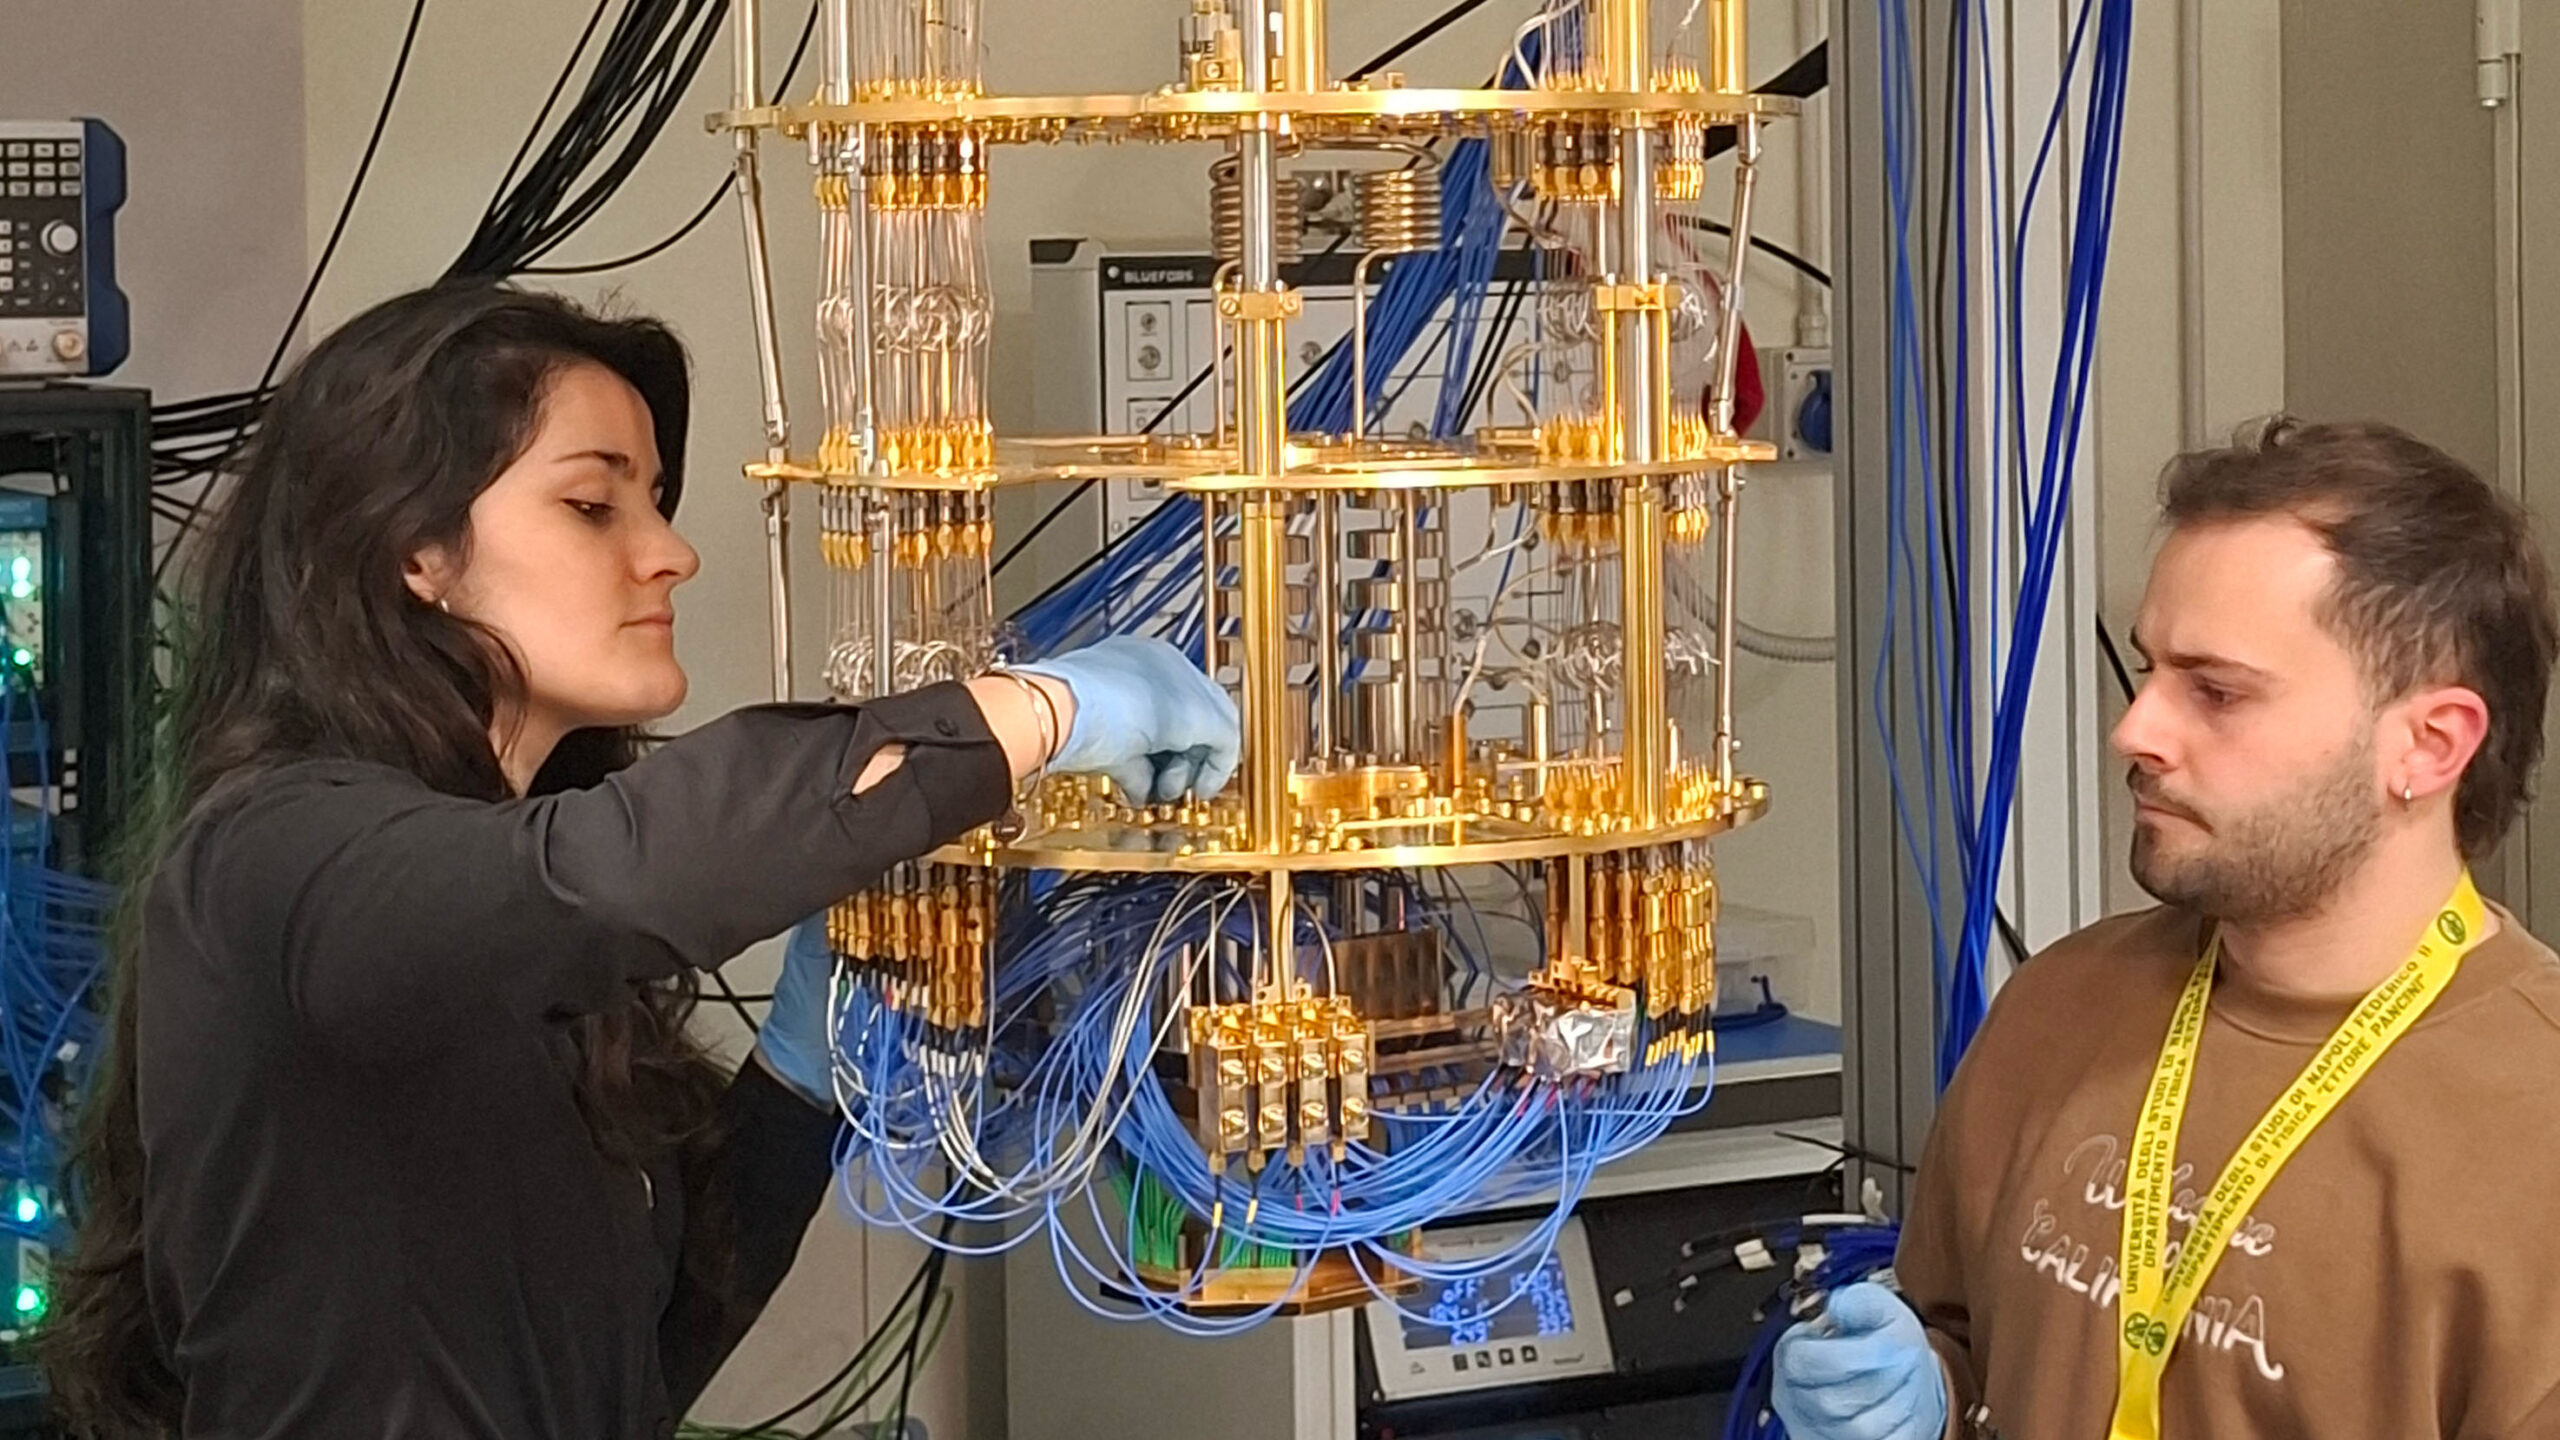
\includegraphics[width=0.85\textwidth]{assets/chapter-3/partenope.jpg}
  \caption{Ricercatori del Dipartimento di Fisica \textit{Ettore Pancini} al lavoro sul criostato di Partenope durante l'installazione del nuovo processore a 64 qubit (2026). Fonte: ICSC.}
  \label{fig:it-partenope}
\end{figure}

Partenope è finanziata da ICSC con fondi PNRR ed è aperta a ricercatori e
imprese, che possono eseguirvi algoritmi propri. Il progetto di sviluppo
coinvolge anche l'azienda italiana Planckian, di cui si dirà nel
Paragrafo~\ref{sec:it-filiera}.

\subsection{Qolossus 2.0: la fotonica della Sapienza}
\label{subsec:it-qolossus}

Presentato il 9 dicembre 2025, \textbf{Qolossus 2.0} è il primo computer
quantistico fotonico italiano, coordinato dalla Sapienza Università di Roma
nell'ambito dell'ICSC~\cite{sapienza2025qolossus}. Segue la logica descritta
nel Paragrafo~\ref{sec:fotonici}: l'informazione viaggia su singoli fotoni
dentro circuiti ottici, e non serve alcuna criogenia.

L'elemento più significativo è che il cuore della macchina è \textbf{italiano}:
il processore fotonico universale a 12 modi è stato realizzato dall'Istituto
di Fotonica e Nanotecnologie del CNR di Milano (CNR-IFN), con la tecnica della
scrittura mediante laser a femtosecondi. Su questo punto - a differenza dei
superconduttori, dove il chip viene comprato all'estero - la filiera nazionale
è completa.

\begin{figure}[ht]
  \centering
  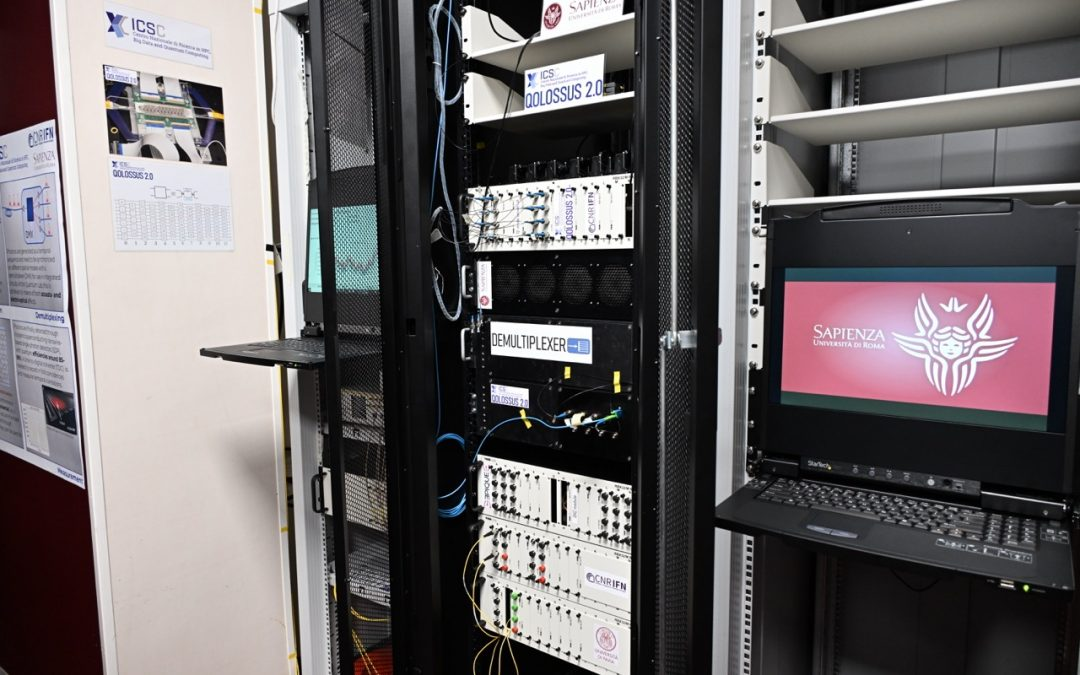
\includegraphics[width=0.85\textwidth]{assets/chapter-3/qolossus.jpg}
  \caption{I rack di Qolossus 2.0 alla Sapienza, con i moduli fotonici etichettati \textit{Qolossus 2.0}, \textit{CNR-IFN} e \textit{Demultiplexer}. Fonte: Sapienza Università di Roma / ICSC.}
  \label{fig:it-qolossus}
\end{figure}

Qolossus 2.0 ha inoltre due caratteristiche poco comuni. È
\textbf{modulare}, cioè pensato per essere ampliato collegando più unità, e
sa lavorare non solo con i qubit ma anche con i \textbf{qudit}, cioè unità di
informazione a più di due livelli: un fotone può essere codificato su molti
modi ottici, e sfruttare questa ricchezza consente di rappresentare più
informazione con lo stesso numero di particelle. Il gruppo della Sapienza,
insieme al Politecnico di Milano e al CNR, sta lavorando alle versioni
successive del processore, con connessioni coerenti tra moduli e iniezione
adattiva dei fotoni in tempo reale.

\subsection{Atomi neutri a Firenze}
\label{subsec:it-firenze}

Il 1\textsuperscript{o} aprile 2026 è stata inaugurata al Campus Scientifico
di Sesto Fiorentino la piattaforma di calcolo quantistico ad \textbf{atomi
neutri} del CNR, realizzata dall'Istituto Nazionale di Ottica (CNR-INO)
insieme al Dipartimento di Fisica e Astronomia dell'Università di
Firenze~\cite{cnr2026atomineutri}.

\begin{figure}[ht]
  \centering
  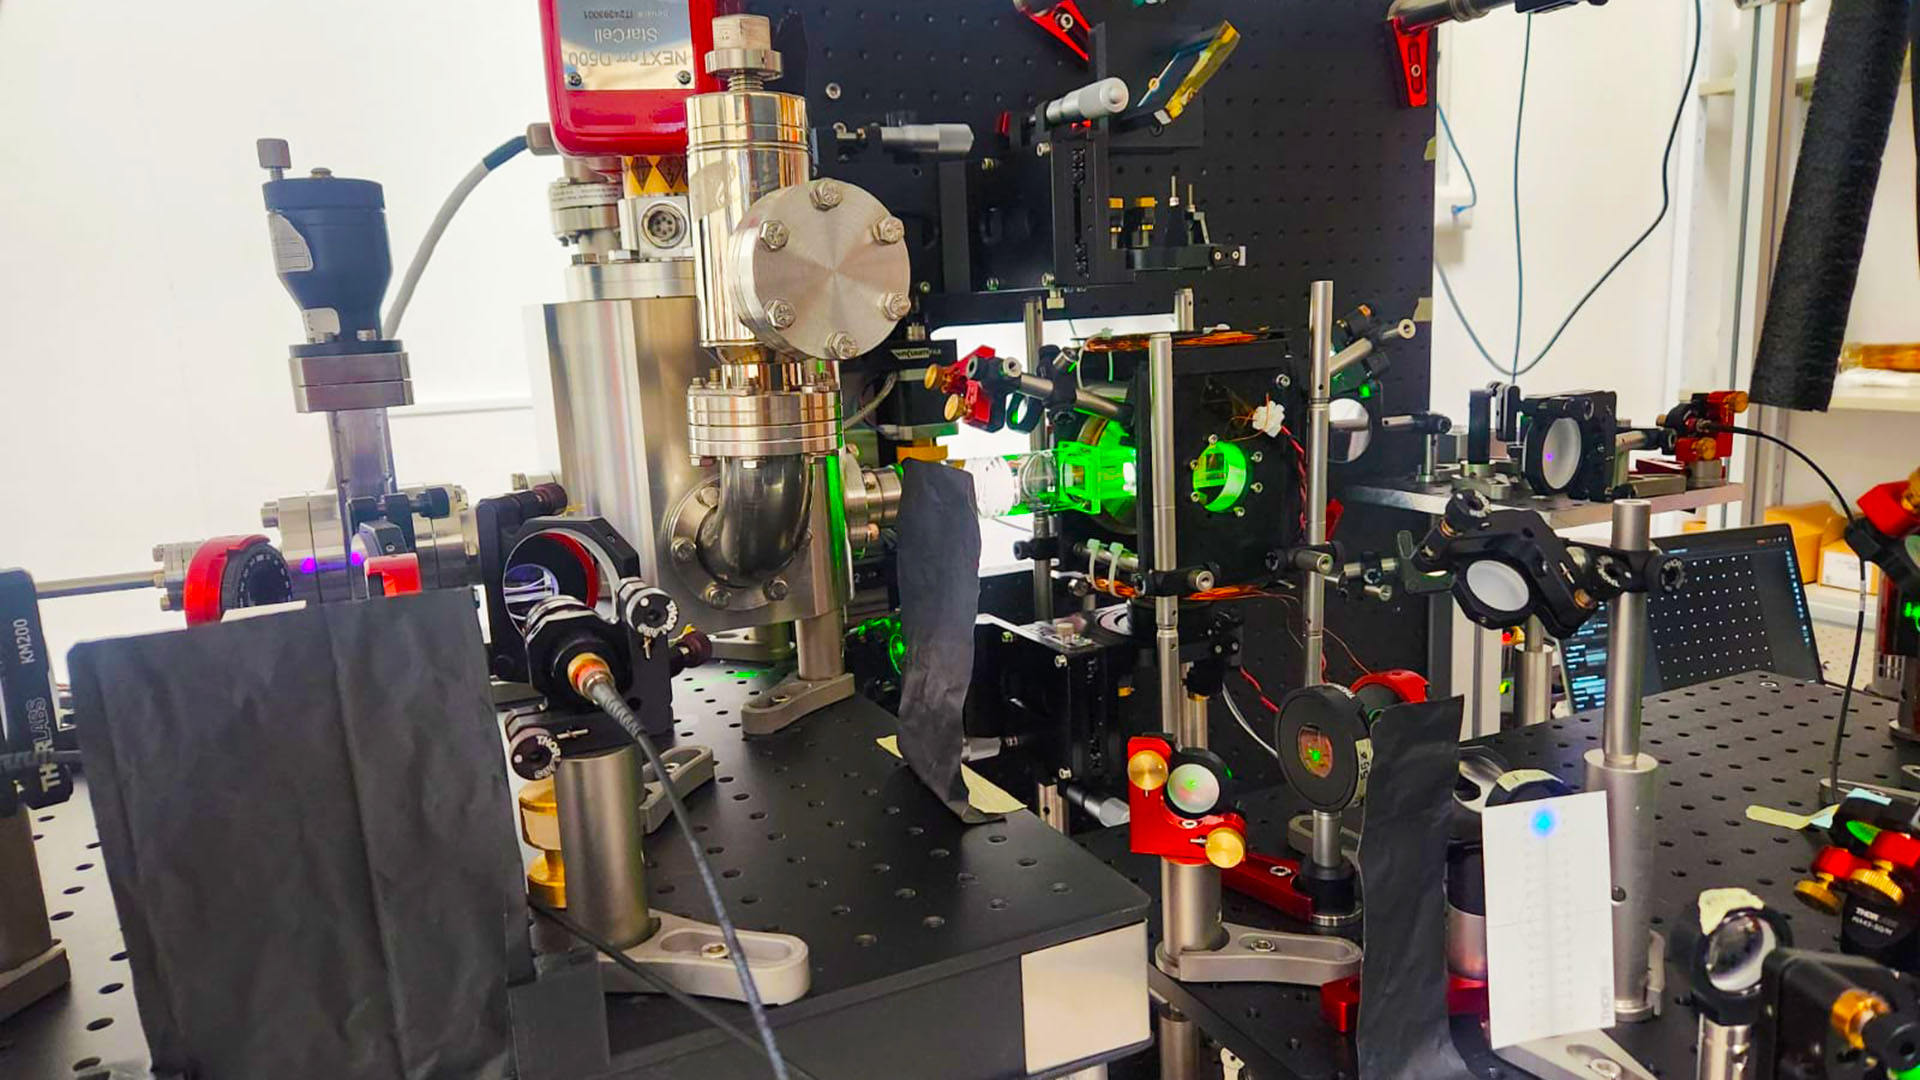
\includegraphics[width=0.85\textwidth]{assets/chapter-3/firenze-atomi.jpg}
  \caption{Il banco ottico della piattaforma ad atomi neutri del CNR a Sesto Fiorentino, con la camera a vuoto, le ottiche e i fasci laser. Fonte: ICSC / CNR.}
  \label{fig:it-firenze}
\end{figure}

Il principio è affine a quello delle trappole ioniche del
Paragrafo~\ref{sec:trap}, ma con una differenza importante: gli atomi qui sono
\textbf{neutri}, non ionizzati, e vengono tenuti fermi da \textit{pinzette
ottiche}, cioè fasci laser fortemente focalizzati che funzionano come piccole
pinze di luce. Non respingendosi tra loro, gli atomi neutri si possono
impacchettare in griglie regolari molto dense, il che rende questa piattaforma
particolarmente promettente sul piano della scalabilità. Per farli interagire -
e quindi realizzare le porte a due qubit - si eccitano gli atomi in stati di
\textbf{Rydberg}, stati in cui l'elettrone più esterno è così lontano dal
nucleo che l'atomo diventa enorme e sente i propri vicini.

La piattaforma fiorentina nasce già con un'architettura dichiaratamente
scalabile, predisposta per arrivare a diverse centinaia di qubit, ed è
finanziata dallo Spoke 10 di ICSC con il concorso di NQSTI. Vale la pena
notare la coincidenza: è la stessa tecnologia della macchina francese
installata a Bologna di cui si parla nel Paragrafo~\ref{sec:it-ospitate}. In
un caso l'Italia la compra, nell'altro la costruisce.

\subsection{Ioni intrappolati a Padova}
\label{subsec:it-padova}

Il 2 marzo 2026 l'Università di Padova ha inaugurato il proprio \textbf{Quantum
Computing Lab}, dedicato a un calcolatore a \textbf{ioni intrappolati} - la
tecnologia con le fedeltà di porta più alte in assoluto, descritta nel
Paragrafo~\ref{sec:trap}~\cite{unipd2026lab}.

Qui il dato interessante non è il numero di qubit, che la macchina svilupperà
nel tempo, ma l'entità dell'investimento infrastrutturale: 4,8 milioni di euro
complessivi, di cui circa 4,5 per la sola strumentazione scientifica (3,5
milioni da fondi WCRI e 1 milione dal PNRR tramite lo Spoke 10). Il
laboratorio occupa 683 m$^2$ e poggia su una platea antivibrazione di oltre
213 m$^2$.

\begin{figure}[ht]
  \centering
  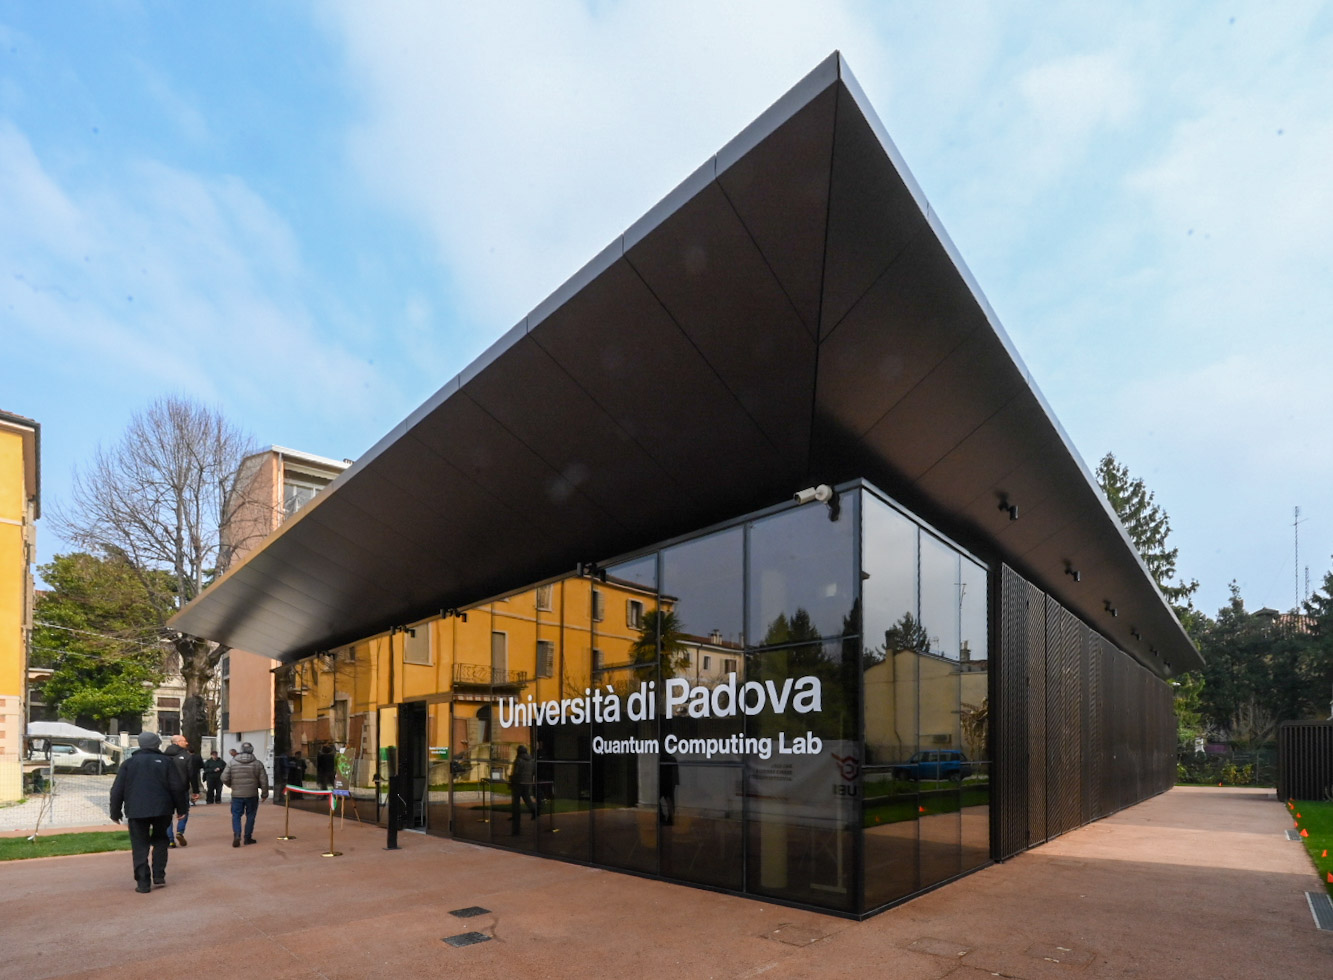
\includegraphics[width=0.85\textwidth]{assets/chapter-3/padova-ioni.jpg}
  \caption{L'edificio del Quantum Computing Lab dell'Università di Padova il giorno dell'inaugurazione (2 marzo 2026). Fonte: Università di Padova.}
  \label{fig:it-padova}
\end{figure}

Quest'ultimo dettaglio dice molto sulla natura del problema. Un calcolatore a
ioni è, in fondo, un insieme di laser puntati su singoli atomi sospesi nel
vuoto: una vibrazione del pavimento è sufficiente a rovinare l'allineamento.
Buona parte del costo di queste macchine non sta nei qubit, ma nell'edificio
che li circonda. Al progetto partecipano dodici dipartimenti dell'ateneo
patavino insieme a CINECA, INFN e alle università di Pavia, L'Aquila, Napoli e
Bologna.

% ─────────────────────────────────────────────────────────────────────────────
\section{Le macchine che l'Italia ospita}
\label{sec:it-ospitate}
% ─────────────────────────────────────────────────────────────────────────────

Accanto alle piattaforme costruite in casa ci sono due sistemi commerciali
acquistati all'estero e installati in Italia. Non sono tecnologia italiana, ma
sono le macchine con cui, oggi, ricercatori e imprese italiane calcolano
davvero.

\paragraph{SOL, il sistema europeo di Bologna.}
Il più potente è \textbf{SOL}, un processore ad atomi neutri da \textbf{140
qubit} costruito dalla francese Pasqal e consegnato il 17 febbraio 2026 al
Tecnopolo DAMA di Bologna, presso il CINECA; l'inaugurazione ufficiale è
avvenuta l'11 giugno 2026~\cite{pasqal2026sol}. SOL è il primo sistema di
calcolo quantistico dell'infrastruttura europea EuroHPC a entrare in funzione,
nell'ambito del consorzio \textbf{EuroQCS-Italy} guidato da CINECA con la rete
accademica slovena ARNES e il centro tedesco Forschungszentrum Jülich, con un
investimento di circa 13 milioni di euro cofinanziato dall'impresa comune
EuroHPC e dal MUR attraverso ICSC.

L'aspetto più rilevante non è però il conteggio dei qubit, ma
l'\textbf{integrazione}: SOL è affiancato a Leonardo, il supercomputer
pre-exascale del CINECA tra i primi dieci al mondo, in un'architettura ibrida
in cui la parte classica e quella quantistica cooperano sullo stesso problema.
La macchina opera attualmente in \textit{modalità analogica} - i qubit
evolvono con continuità sotto l'azione dei laser, invece di eseguire una
sequenza di porte discrete - ed è previsto per il 2027 un aggiornamento che
abiliterà anche il funzionamento digitale~\cite{cineca2026euroqcs}.

\paragraph{Il piccolo IQM di Torino.}
Il 22 maggio 2025 è stato acceso al Politecnico di Torino, in collaborazione
con la Fondazione LINKS e l'INRiM, il primo computer quantistico della
finlandese IQM installato in Italia: \textbf{cinque qubit} superconduttori
raffreddati a 20\,mK~\cite{inrim2025iqm}. Cinque qubit non risolvono alcun
problema pratico, e sarebbe fuorviante presentarlo come una macchina di
calcolo. Il suo valore è diverso: è un sistema completo, reale e
\textbf{accessibile}, su cui studenti, ricercatori e aziende possono imparare
a lavorare senza passare dal cloud di un fornitore straniero. L'INRiM, in
particolare, lo usa per sviluppare strumenti di misura destinati a migliorare
le prestazioni dei qubit superconduttori: un ruolo da istituto metrologico,
coerente con la sua missione.

\begin{figure}[ht]
  \centering
  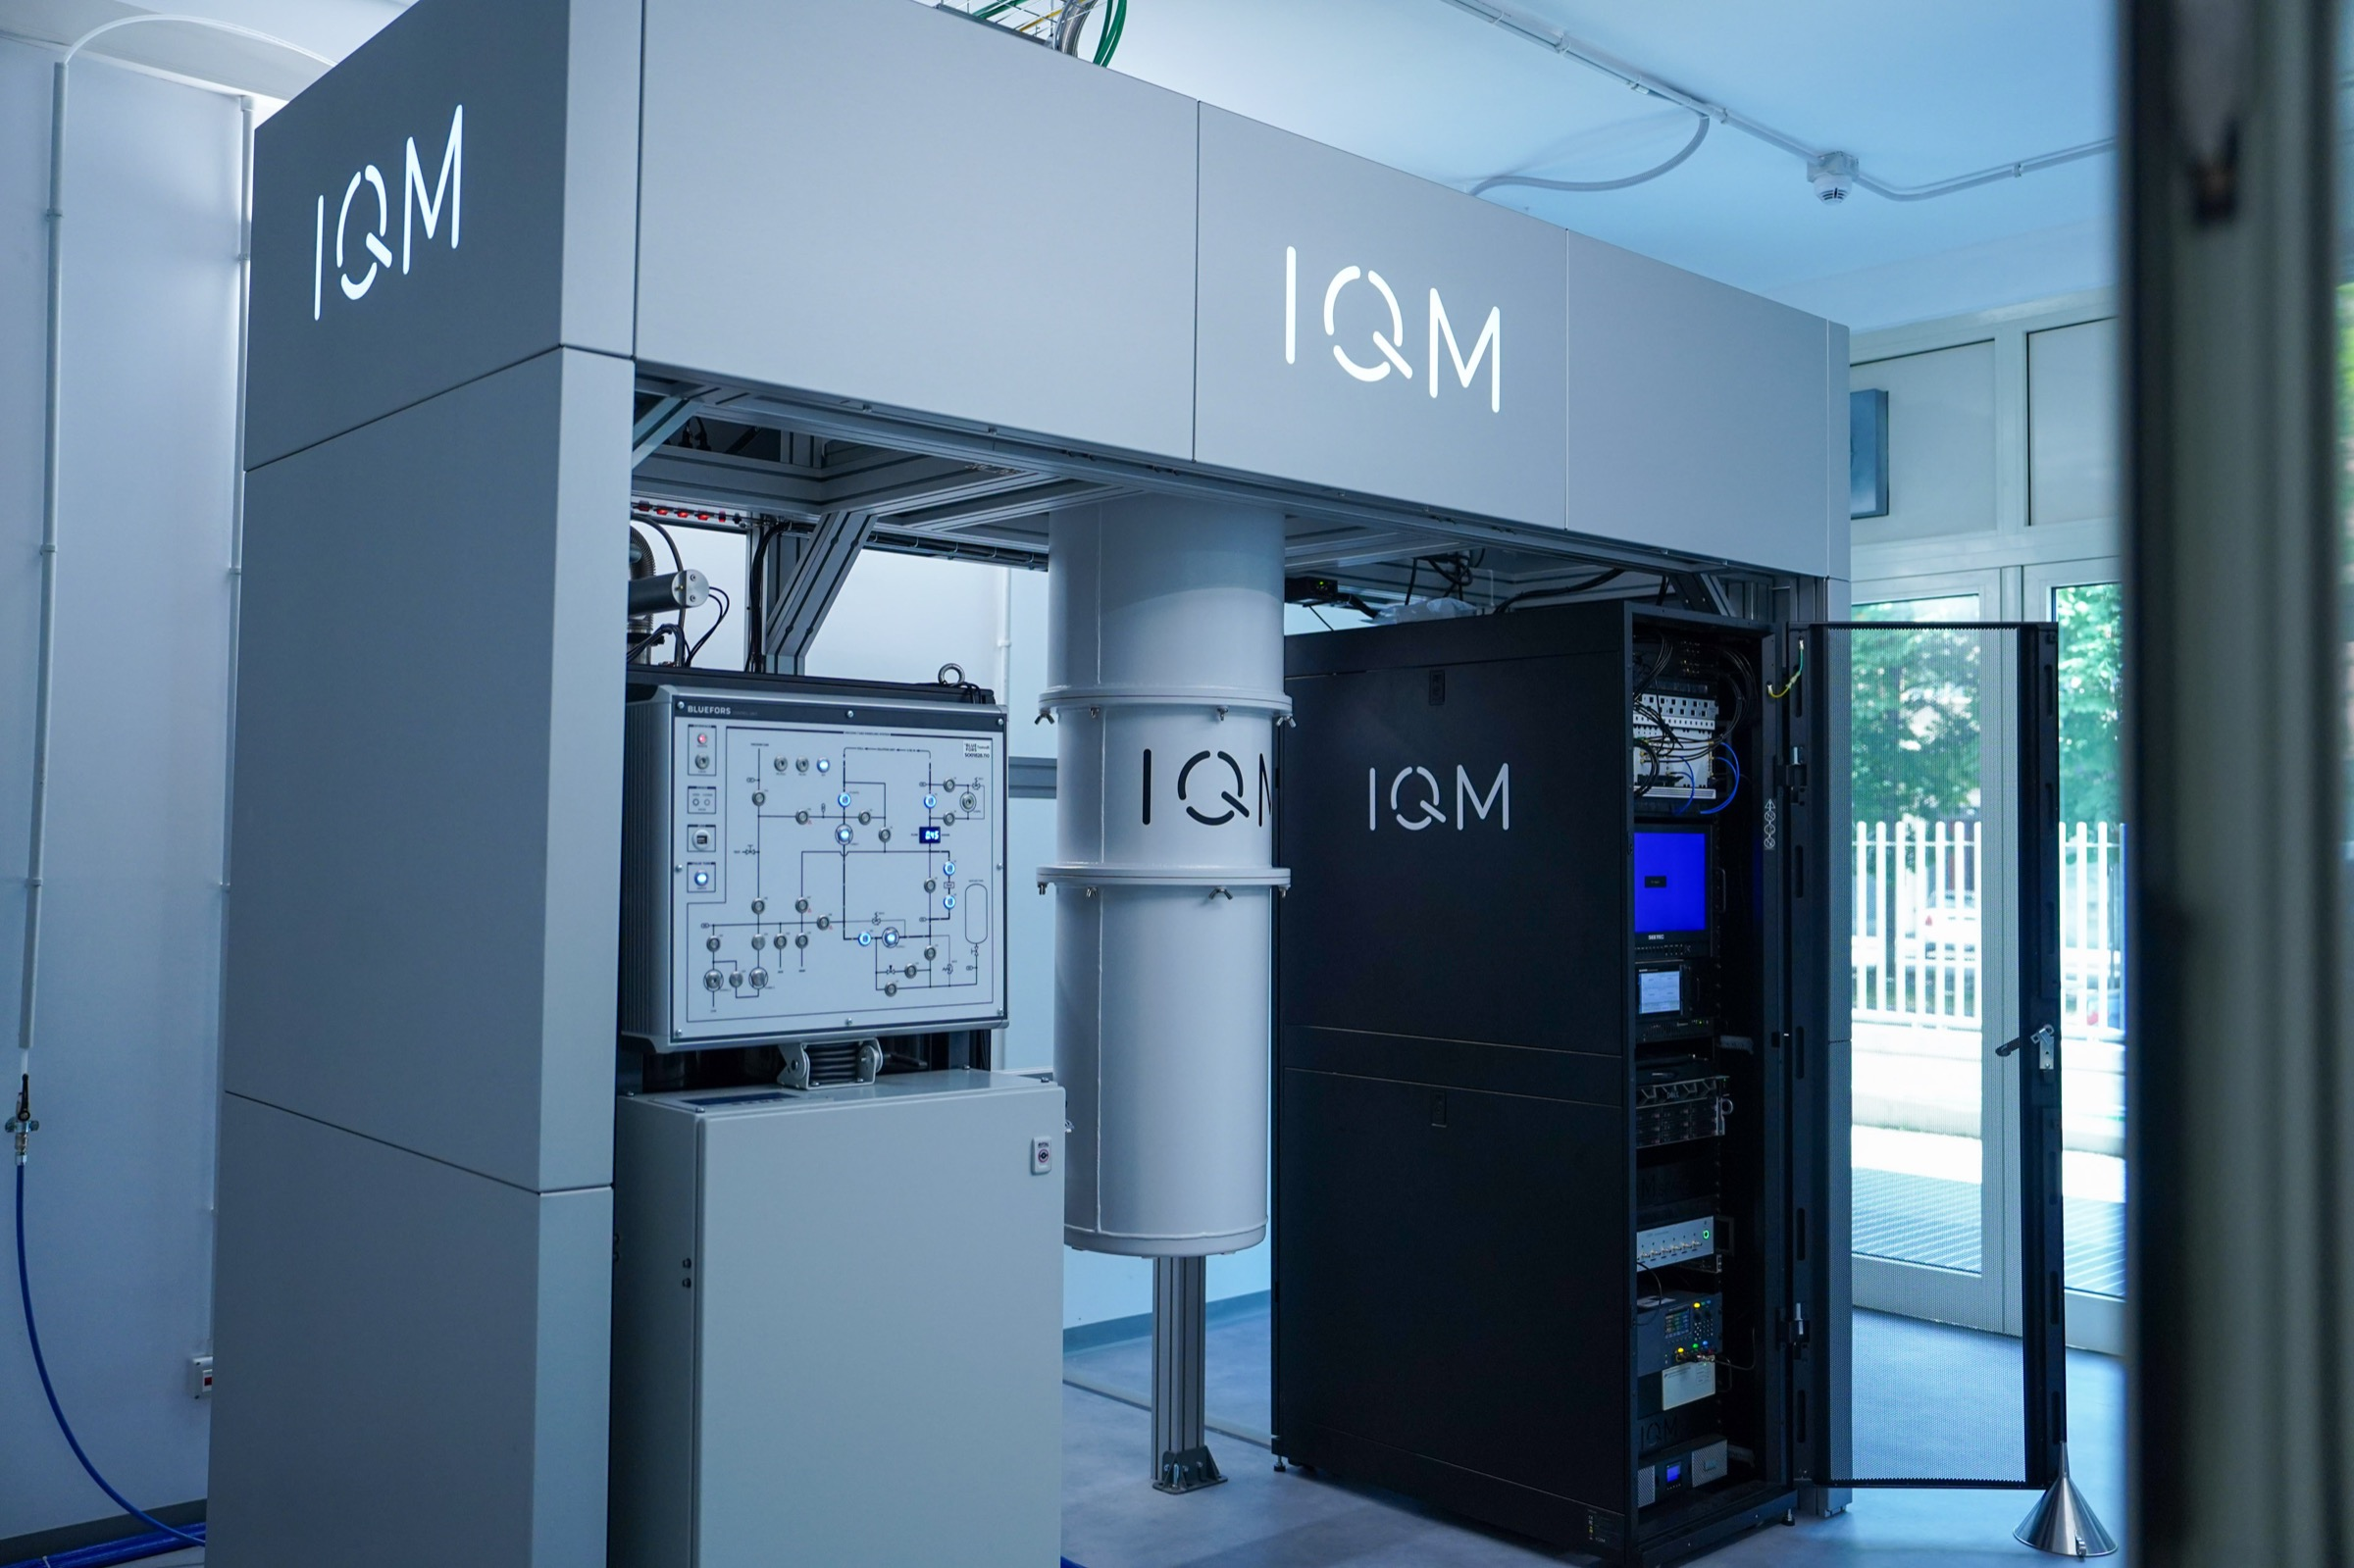
\includegraphics[width=0.85\textwidth]{assets/chapter-3/iqm-torino.jpg}
  \caption{Il computer quantistico IQM a 5 qubit nel data center del Politecnico di Torino: al centro il criostato (il cilindro bianco), a sinistra il pannello del sistema di raffreddamento e a destra il rack dell'elettronica di controllo. Fonte: Politecnico di Torino.}
  \label{fig:it-iqm}
\end{figure}

% ─────────────────────────────────────────────────────────────────────────────
\section{La filiera dei componenti}
\label{sec:it-filiera}
% ─────────────────────────────────────────────────────────────────────────────

Il terzo livello è il meno visibile e forse il più importante nel lungo
periodo: chi, in Italia, fabbrica i pezzi.

\paragraph{Il primo qubit superconduttivo made in Italy.}
Nel 2024 la Fondazione Bruno Kessler di Trento ha realizzato il primo qubit
superconduttivo interamente costruito in Italia: un transmon basato su
giunzioni Josephson in alluminio, con barriere spesse circa un milionesimo di
millimetro, progettato dal gruppo coordinato da Federica Mantegazzini insieme
ai ricercatori dell'INFN di Milano-Bicocca~\cite{fbk2024qubit}. Il risultato
non ha valore prestazionale - un singolo qubit non calcola nulla - ma
strategico: rompe la dipendenza dall'importazione dei dispositivi.

\paragraph{Dal qubit singolo alla catena nazionale.}
Il 15 luglio 2026 quel percorso ha fatto un passo ulteriore. Presso il
laboratorio COLD dei Laboratori Nazionali di Frascati dell'INFN è stato
caratterizzato con successo un \textbf{transmon 3D} in alluminio, fabbricato
dal CNR-IFN di Roma nell'infrastruttura NanoMicroFab di Tor Vergata e
alloggiato in una cavità superconduttiva realizzata ai Laboratori Nazionali di
Legnaro~\cite{cnr2026transmon}. Ogni anello della catena - progetto,
fabbricazione, cavità, misura - è italiano.

Il dispositivo mantiene la coerenza per circa \textbf{un quarto di
microsecondo}. Vale la pena essere espliciti su cosa significhi questo numero:
è due o tre ordini di grandezza al di sotto dei transmon commerciali, che
superano abitualmente i 100\,$\mu$s. Non siamo davanti a un record, ma alla
validazione di una filiera che prima non esisteva. Il progetto nasce del resto
con un obiettivo diverso dal calcolo: usare i qubit come sensori per la fisica
fondamentale, in particolare nella ricerca della materia oscura assionica,
nell'ambito dei progetti Qub-IT e Quartet dell'INFN insieme a ICSC, NQSTI e
all'ERC Synergy GravNet.

\paragraph{Ephos: i chip fotonici in vetro.}
Fondata nel 2022 e nata nell'ecosistema del CNR e del Politecnico di Milano,
\textbf{Ephos} produce circuiti fotonici scritti dentro il \textit{vetro}
anziché sul silicio, ottenendo perdite ottiche molto basse - una qualità
decisiva quando il segnale è costituito da singoli fotoni. Dopo un round seed
da 8,5 milioni di dollari, con la partecipazione dello European Innovation
Council e dell'acceleratore DIANA della NATO, nel luglio 2025 l'azienda ha
ottenuto \textbf{41,5 milioni di euro} dal MIMIT nell'ambito dello EU Chips
Act - primo finanziamento del genere concesso a una startup - per costruire
nell'area milanese \textit{Fab-2}, primo impianto al mondo dedicato alla
lavorazione di wafer di vetro, a fronte di un investimento complessivo di
104,9 milioni~\cite{mimit2025ephos}.

\paragraph{Planckian: risolvere il problema dei cavi.}
Nata nel 2023 come primo spin-off congiunto dell'Università di Pisa e della
Scuola Normale Superiore, \textbf{Planckian} lavora su un problema molto
concreto dei processori superconduttori: il \textbf{cablaggio}. Come si è
visto nel Paragrafo~\ref{subsec:nv-cmos} a proposito del diamante, ogni qubit
richiede in linea di principio la propria linea di controllo, e dentro un
criostato ogni cavo in più significa ingombro e calore. L'architettura
proposta da Planckian consente a più qubit di \textbf{condividere le linee di
controllo}, riducendo la complessità criogenica~\cite{planckian2026}. La
società collabora con il QTLab della Federico II e, dal 2026, con Quantum
Elements per la modellazione del rumore a fini di correzione d'errore.

\paragraph{QTI: la rete, non il calcolo.}
Per completezza va citata \textbf{QTI} (\textit{Quantum Telecommunications
Italy}), spin-off del CNR-INO nata a Firenze nel 2020 e oggi controllata da
Telsy del gruppo TIM. QTI non costruisce computer ma sistemi industriali di
\textbf{distribuzione quantistica di chiavi} (QKD): è il ramo delle
comunicazioni quantistiche, complementare al calcolo, e rappresenta il caso
italiano più maturo di trasferimento dalla ricerca al prodotto.

% ─────────────────────────────────────────────────────────────────────────────
\section{E il diamante?}
\label{sec:it-diamante}
% ─────────────────────────────────────────────────────────────────────────────

Dato che questa tesi è dedicata ai centri NV nel diamante, la domanda è
d'obbligo. La risposta onesta è che \textbf{in Italia non esiste un computer
quantistico a centri NV}, né un progetto dichiarato per costruirne uno. Il
contributo italiano al diamante quantistico è di altra natura, e si concentra
su due fronti.

\paragraph{La fotonica del diamante.}
Il CNR-IFN di Milano, con il gruppo di Shane Eaton, ha sviluppato insieme
all'Università di Ulm un metodo ibrido per portare i qubit \textit{dentro} i
circuiti ottici scavati nel diamante: la scrittura con laser a femtosecondi
crea guide d'onda tridimensionali nel cristallo, e un fascio ionico impianta
poi i centri di colore nella posizione voluta. Il lavoro, pubblicato su
\textit{ACS Photonics}, dimostra l'accoppiamento di singoli centri
\textbf{SiV} (\textit{silicon-vacancy}, a lacuna di silicio) a una guida
d'onda scritta al laser~\cite{eaton2022siv}. Il centro SiV è un cugino
dell'NV: stesso tipo di difetto, ma con l'azoto sostituito dal silicio, il che
gli conferisce proprietà ottiche migliori a scapito della coerenza a
temperatura ambiente. È la stessa competenza di scrittura laser che sta dietro
al processore fotonico di Qolossus e alla tecnologia di Ephos.

\paragraph{La sensoristica.}
L'altro fronte è quello descritto nel Paragrafo~\ref{sec:nv-applicazioni}:
usare il centro NV non per calcolare ma per misurare. L'INRiM lavora da anni
sulla metrologia quantistica basata su centri NV, mentre l'Agenzia Spaziale
Italiana partecipa al progetto europeo ACDC\_Q, che punta a miniaturizzare i
sensori NV per la magnetometria spaziale sostituendo l'ingombrante apparato
ottico da laboratorio con elettronica a semiconduttore~\cite{asi2025acdcq}. È
lo stesso movimento concettuale del chip cryo-CMOS descritto nel
Paragrafo~\ref{subsec:nv-cmos}: portare il controllo del centro NV dentro un
circuito integrato.

\begin{notabox}
  Il posizionamento italiano sul diamante è quindi coerente con la storia
  scientifica del Paese: forte sull'\textbf{ottica} e sulla
  \textbf{metrologia}, debole sull'integrazione di sistema. L'Italia sa
  scrivere circuiti dentro il diamante e sa misurare con i centri NV; non ha
  però - almeno per ora - il tipo di investimento industriale che servirebbe
  per trasformare quelle competenze in un calcolatore.
\end{notabox}

% ─────────────────────────────────────────────────────────────────────────────
\section{Quadro d'insieme}
\label{sec:it-quadro}
% ─────────────────────────────────────────────────────────────────────────────

La Tabella~\ref{tab:it-macchine} riassume le macchine oggi operative o in
allestimento sul territorio italiano.

\begin{table}[ht]
  \centering
  \renewcommand{\arraystretch}{1.3}
  \caption{Sistemi di calcolo quantistico in Italia (situazione a metà 2026).}
  \label{tab:it-macchine}
  \begin{tabularx}{\textwidth}{>{\bfseries}lXXXl}
    \toprule
    Sistema & Sede & Tecnologia & Scala & Origine \\
    \midrule
    SOL          & CINECA, Bologna    & Atomi neutri      & 140 qubit    & Acquistata \\
    Partenope    & Federico II, Napoli & Superconduttori  & 64 qubit     & Mista \\
    Qolossus 2.0 & Sapienza, Roma     & Fotonica          & 12 modi      & Italiana \\
    (in avvio)   & CNR-INO, Firenze   & Atomi neutri      & Scalabile    & Italiana \\
    (in avvio)   & UniPD, Padova      & Ioni intrappolati & In sviluppo  & Italiana \\
    IQM          & PoliTo, Torino     & Superconduttori   & 5 qubit      & Acquistata \\
    \bottomrule
    \multicolumn{5}{l}{\footnotesize \textit{Mista}: sistema integrato in Italia con processore di fornitore estero.} \\
  \end{tabularx}
\end{table}

Letta nel suo insieme, la tabella racconta tre cose. La prima è che la
macchina più potente installata in Italia non è italiana: il divario di scala
tra i 140 qubit di SOL e le piattaforme nazionali è netto. La seconda è che
l'unica riga interamente italiana dal processore in su è quella fotonica di
Roma, non a caso il campo in cui il Paese ha la tradizione più solida. La
terza è che tre delle sei voci sono entrate in funzione tra dicembre 2025 e
giugno 2026: il panorama è appena nato, e qualunque fotografia invecchia in
fretta.

% ─────────────────────────────────────────────────────────────────────────────
\section{Conclusioni del Capitolo}
\label{sec:it-conclusioni}
% ─────────────────────────────────────────────────────────────────────────────

L'Italia è entrata nel calcolo quantistico tardi e con risorse limitate, ma
con una strategia riconoscibile: non inseguire il numero di qubit, bensì
costruire in parallelo quattro piattaforme di ricerca, ospitare le macchine
europee più potenti e alimentare una filiera nazionale di componenti.

I punti di forza sono quelli storici della fisica italiana. L'ottica
quantistica di Firenze, Roma e Milano ha prodotto l'unico processore
interamente nazionale; la metrologia dell'INRiM presidia il terreno della
misura, indispensabile per migliorare qualunque qubit; la fabbricazione
micro-nanometrica di FBK, CNR-IFN e INFN ha dimostrato di saper produrre
dispositivi superconduttivi in casa. Attorno a queste competenze sta nascendo
un piccolo tessuto industriale - Ephos, Planckian, QTI - che tra il 2024 e il
2025 ha raccolto decine di milioni di euro.

Le fragilità sono altrettanto chiare. I processori superconduttori più
performanti si comprano ancora all'estero; le prestazioni dei dispositivi
nazionali, come il quarto di microsecondo del transmon di Frascati, sono
lontane dallo stato dell'arte; e soprattutto l'intera impalcatura poggia su
fondi PNRR in esaurimento, senza che sia ancora definito con quali risorse
ordinarie si manterranno le infrastrutture appena inaugurate.

Rispetto al tema di questa tesi, infine, il bilancio è asimmetrico: l'Italia
partecipa al diamante quantistico con contributi di rilievo sulla fotonica e
sulla sensoristica, ma non sul calcolo. Se il diamante diventerà una
piattaforma di calcolo credibile - e il Capitolo~\ref{chap:implementazioni} ha
mostrato che la strada passa dall'integrazione cryo-CMOS e dai collegamenti
fotonici tra centri NV - le competenze italiane si collocano esattamente sui
componenti che serviranno, ma non sulla macchina che li metterà insieme.
